\documentclass[FCD_GNN.tex]{subfiles}

\begin{document}
\chapter{Method}
\label{chapter:Method}
As mentioned earlier, the design of our architecture was inspired by the work of~\cite{Zhong2023Ariadne}. 
The key differences in our implementation are threefold: 
(1) we increase the number of feature extraction layers, 
(2) we introduce a GNN-based block to better aggregate visual features at the top layers, 
and (3) we disable the text branch in the final decoder layers to reduce overfitting. 
The overall architecture is illustrated in Figure~\ref{fig:architecture}, 
and each component is described in more detail below.

\begin{figure}[htbp]
    \centering
    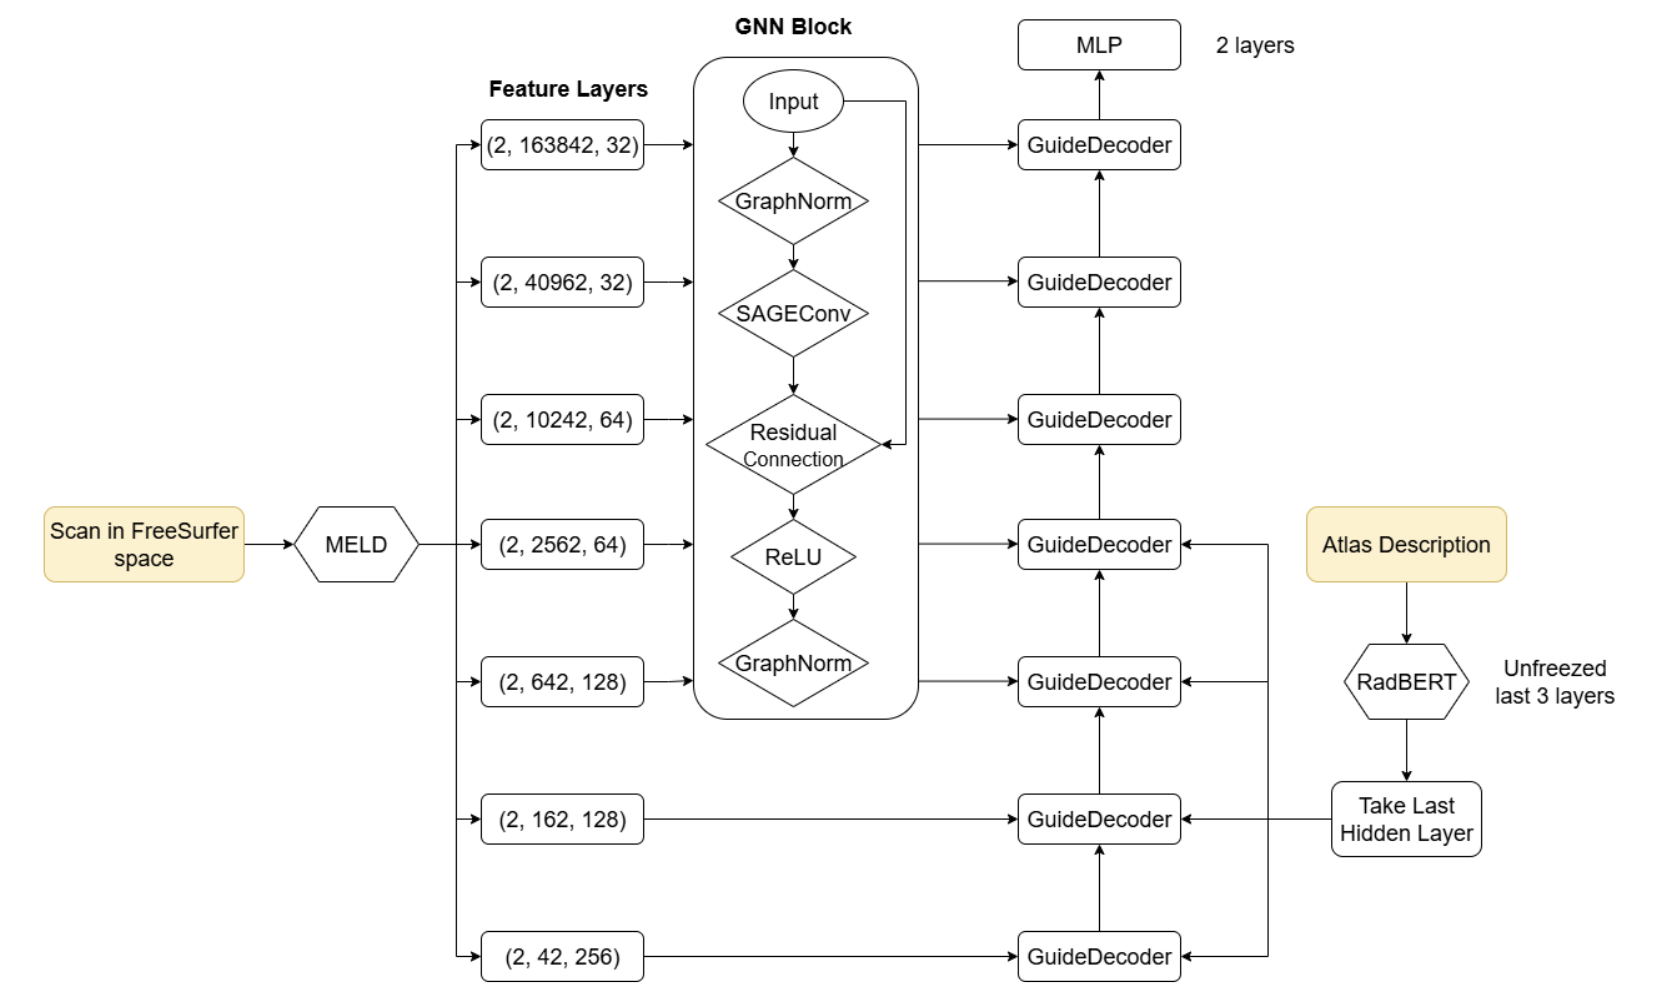
\includegraphics[width=1.0\textwidth]{architecture.png}
    \caption{Overview of the proposed multimodal segmentation architecture. 
    Visual features extracted from FreeSurfer surface space are processed through hierarchical GNN layers, 
    while textual embeddings from RadBERT guide the decoder via cross-attention.}
    \label{fig:architecture}
\end{figure}

\section{Visual Feature Extraction}

As input to the vision model, structural MRI scans are first mapped into the FreeSurfer surface space.  
From the \ac{meld} preprocessing pipeline, we obtain a multi-resolution set of surface-based features across 
seven hierarchical levels. Each level is represented as a tensor of shape $(H, N, C)$, where:  

\begin{itemize}
    \item $H$ – number of hemispheres (left/right),
    \item $N$ – number of vertices on the cortical mesh per hemisphere,
    \item $C$ – number of features per vertex.
\end{itemize}

To aggregate higher-order geometric information, we process the \textbf{five top feature layers} individually through a dedicated \textbf{GNN Block}.  
This choice is motivated by empirical findings (see Chapter~\ref{chapter:Experiments}), where including the lowest two layers led to oversmoothing and diluted 
discriminative information, while the top five layers yielded the best trade-off between expressivity and stability.  

\section{GNN Block}

Formally, let 
\[
\mathbf{X}^{(l)} \in \mathbb{R}^{(B \cdot H \cdot N_l) \times C_l}
\]
denote the input feature matrix at layer $l$, where 
$B$ is the batch size, 
$H$ is the number of hemispheres, 
$N_l$ is the number of vertices per hemisphere at layer $l$, 
and $C_l$ is the number of input channels.  

Each \textit{GNN Block} then applies the following sequence of operations:

\begin{align}
    \mathbf{H}_0 &= \operatorname{GraphNorm}\!\left(\mathbf{X}^{(l)}, \texttt{batch}\right), \\[4pt]
    \mathbf{H}_1 &= \operatorname{SAGEConv}\!\left(\mathbf{H}_0, \texttt{edge\_index}_l\right), \\[4pt]
    \mathbf{H}_2 &= \mathbf{H}_1 + \mathbf{H}_0 \quad \text{(residual connection)}, \\[4pt]
    \mathbf{H}_3 &= \operatorname{ReLU}\!\left(\mathbf{H}_2\right), \\[4pt]
    % \mathbf{H}_4 &= \operatorname{Dropout}\!\left(\mathbf{H}_3\right), \\[4pt]
    % \mathbf{Z}^{(l)} &= \operatorname{GraphNorm}\!\left(\mathbf{H}_4, \texttt{batch}\right).
    \mathbf{Z}^{(l)} &= \operatorname{GraphNorm}\!\left(\mathbf{H}_3, \texttt{batch}\right).
\end{align}

\noindent\textbf{where:}
\begin{itemize}
    \item $\mathbf{X}^{(l)} \in \mathbb{R}^{(B \cdot H \cdot N_l)\times C_l}$ — input feature matrix at level $l$;
    \item $\texttt{edge\_index}_l \in \mathbb{N}^{2\times |E_l|}$ — adjacency structure of the cortical surface graph;
    \item $\texttt{batch}$ — batch vector;
    \item $\mathbf{Z}^{(l)} \in \mathbb{R}^{(B \cdot H \cdot N_l)\times C_l}$ — resulting representation for level $l$;
    \item $\operatorname{\textbf{SAGEConv}}$ implements the GraphSAGE~\cite{Hamilton2017GraphSAGE} update rule
    \[
    \mathbf{x}_i' = \mathbf{W}_1 \mathbf{x}_i + \mathbf{W}_2 \cdot \underset{j \in \mathcal{N}(i)}{\operatorname{mean}} \text{ } \mathbf{x}_j,
    \]
    where $\mathcal{N}(i)$ is the neighborhood of node $i$;
    \item $\operatorname{\textbf{GraphNorm}}(x) = \gamma \cdot \dfrac{x - \mu_g}{\sqrt{\sigma_g^2+\epsilon}} + \beta$, where $\mu_g, \sigma_g^2$ are mean and variance per graph, and $\gamma,\beta$ are learnable parameters;
    \item $\operatorname{\textbf{ReLU}}(x) = \max(0, x)$ — rectified linear activation function;
    \item $\operatorname{\textbf{Dropout}}(x)$ randomly sets a subset of elements in $x$ to zero with probability $p$.
\end{itemize}

After passing through the GNN Block, the feature dimensionality remains unchanged, ensuring consistency with subsequent blocks. The resulting features are then passed to the GuideDecoder for multimodal fusion.

\section{Textual Feature Extraction}

The text branch of our architecture leverages the pretrained \textbf{RadBERT} model~\cite{Park2022AIforNeuro}, which is specifically designed for radiology reports.   
Prior studies have demonstrated that selectively unfreezing the last few layers of transformer models can improve downstream performance compared to freezing the entire model~\cite{Peters2019ToTune}.  
Motivated by this insight, we unfreeze the last 3 hidden layers of RadBERT—this specific choice is justified in Chapter~\ref{chapter:Experiments}.  
The output of the (now trainable) final hidden layer is then forwarded to each GuideDecoder for multimodal fusion, except for the topmost three layers.

\section{GuideDecoder}
We adopt the GuideDecoder architecture proposed by Zhong et al.~\cite{Zhong2023Ariadne}, 
which fuses visual and textual features in a multi–modal fashion. 
The decoder first projects the textual tokens to align their dimensionality with 
that of the visual tokens, then applies \texttt{multi–head self–attention} and \texttt{cross–attention} 
to exchange semantic information across modalities. 
Finally, the fused features are upsampled and combined with skip connections 
from the visual encoder at the same resolution before the final prediction.

In our implementation, the overall design of the GuideDecoder is preserved, 
but we introduce two modifications to adapt the architecture to surface–based representations. 
First, we replace the standard 2D upsampling with the \texttt{HexUnpool} operator 
(see Appendix~\nameref{sec:hexunpool}), which performs mean unpooling on the icosphere mesh. 
Second, after upsampling and fusion with skip connections, the features are processed by a convolutional 
block based on \texttt{DynUNetBlock} (\href{https://docs.monai.io/en/0.3.0/_modules/monai/networks/blocks/dynunet_block.html}{Code link}) from the MONAI framework, which applies a sequence of convolution, normalization, 
and activation layers. In our architecture, we replace this module with a custom \texttt{SpiralConv-based block} 
that operates on the surface mesh representation of the cortex. 
\end{document}
